% XCircuit output "BJT_koncentracie_vsetky_rezimy.tex" for LaTeX input from BJT_koncentracie_vsetky_rezimy.ps
\def\putbox#1#2#3#4{\makebox[0in][l]{\makebox[#1][l]{}\raisebox{\baselineskip}[0in][0in]{\raisebox{#2}[0in][0in]{\scalebox{#3}{#4}}}}}
\def\rightbox#1{\makebox[0in][r]{#1}}
\def\centbox#1{\makebox[0in]{#1}}
\def\topbox#1{\raisebox{-0.60\baselineskip}[0in][0in]{#1}}
\def\midbox#1{\raisebox{-0.20\baselineskip}[0in][0in]{#1}}
   \scalebox{0.8}{
   \normalsize
   \parbox{3.60417in}{
   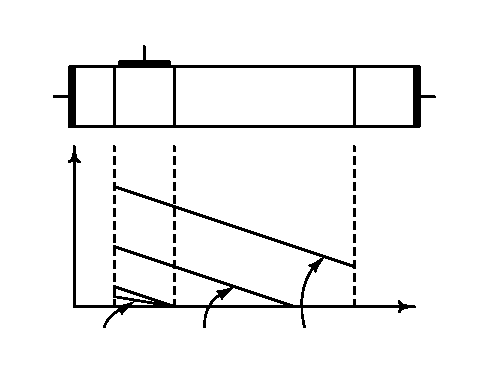
\includegraphics[scale=1.25]{BJT_koncentracie_vsetky_rezimy}\\
   % translate x=383 y=591 scale 0.30
   \putbox{0.19in}{2.11in}{1.20}{E}%
   \putbox{1.00in}{2.61in}{1.20}{B}%
   \putbox{3.52in}{2.11in}{1.20}{C}%
   \putbox{0.52in}{2.06in}{1.20}{N$^+$}%
   \putbox{0.98in}{2.06in}{1.20}{P}%
   \putbox{1.65in}{2.06in}{1.20}{N$^-$- drift}%
   \putbox{2.94in}{2.06in}{1.20}{N$^+$}%
   \putbox{1.90in}{1.06in}{1.20}{$n \approx p$}%
   \putbox{3.06in}{0.23in}{1.20}{$x$}%
   \putbox{0.06in}{1.48in}{1.20}{$n, p$}%
   \putbox{0.65in}{1.31in}{1.20}{F}%
   \putbox{0.65in}{0.81in}{1.20}{F}%
   \putbox{0.65in}{0.48in}{1.20}{F}%
   \putbox{1.36in}{1.23in}{1.20}{F}%
   \putbox{1.36in}{0.73in}{1.20}{F}%
   \putbox{1.36in}{0.40in}{1.20}{R}%
   \putbox{0.52in}{0.06in}{1.20}{aktiv.}%
   \putbox{1.23in}{0.06in}{1.20}{\rotatebox{-360}{kvazi-sat.}}%
   \putbox{2.31in}{0.06in}{1.20}{\rotatebox{-360}{sat.}}%
   \putbox{0.98in}{1.40in}{1.20}{$n$}%
   } % close 'parbox'
   } % close 'scalebox'
   \vspace{-\baselineskip} % this is not necessary, but looks better
